% Autore= \SE{}
\subsubsection{UCS 7 - Monitoraggio degli accessi effettuati}

\begin{itemize}
\item \textbf{Attori primari:} Amministratore visualizzatore
\item \textbf{Precondizione:} L'amministratore dispone di almeno un'\glo{organizzazione}.
\item \textbf{Postcondizione:} L'amministratore ha monitorato gli accessi effettuati dagli utenti riconosciuti.
\item \textbf{Scenario principale:} L'amministratore, dopo aver selezionato l'\glo{organizzazione}, accede alla funzionalità di visualizzazione della \glo{lista degli accessi} per monitorare gli utenti.
\item \textbf{Flusso di eventi:} 
\begin{enumerate}
	\item L'amministratore ha selezionato l'\glo{organizzazione} [UCS 3];
	\item L'amministrazione seleziona la funzionalità di visualizzazione della \glo{lista degli accessi};
	\item L'amministrazione può visualizzare gli accessi effettuati da un utente riconosciuto presso l'\glo{organizzazione} [UCS 7.1] o in un \glo{luogo} all'interno di essa [UCS 7.2].
\end{enumerate}
\end{itemize}

\subsubsection{UCS 7.1 - Visualizzazione degli accessi effettuati da un utente riconosciuto presso l'organizzazione}
\begin{figure}[h]
	\centering
	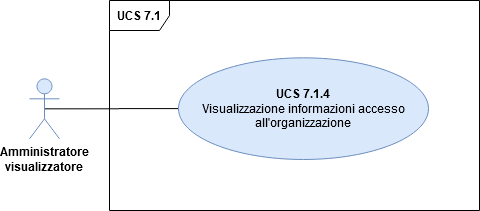
\includegraphics[scale=0.4]{Sezioni/UseCase/Immagini/UCS7.1.png}
	\caption{UCS 7.1 - Visualizzazione degli accessi effettuati da un utente riconosciuto presso l'\glo{organizzazione}}
\end{figure}
\begin{itemize}
	\item \textbf{Attori primari:} Amministratore visualizzatore
	\item \textbf{Precondizione:} L'amministratore ha effettuato l'accesso alla funzionalità di monitoraggio degli accessi effettuati.
	\item \textbf{Postcondizione:} L'amministratore ha visualizzato la lista con gli accessi di un utente riconosciuto presso l'\glo{organizzazione}.
	\item \textbf{Scenario principale:} L'amministratore esegue la procedura per visualizzare lo \glo{storico degli accessi} effettuati presso l'\glo{organizzazione} desiderata da un utente riconosciuto.\\
	L'amministratore può selezionare un luogo all'interno dell'\glo{organizzazione} per monitorare gli accessi dell'utente al suo interno[UCS 7.2].
	\item \textbf{Flusso di eventi:}
	\begin{enumerate}
	\item L'amministratore seleziona un utente preciso da una lista contente tutti i utenti riconosciuti dell'\glo{organizzazione};
	\item L'amministratore visualizza una lista con tutti gli accessi effettuati dall'utente selezionato presso l'\glo{organizzazione};
	\item L'amministratore ha la possibilità di ordinare gli accessi dell'utente all'\glo{organizzazione} [UCS 7.1.1] [UCS 7.1.2] oppure di effettuare una ricerca tra di essi per gli accessi di uno specifico giorno [UCS 7.1.3].
	\end{enumerate}
\end{itemize}

\subsubsection{UCS 7.1.1 - Ordinamento per data decrescente della lista degli accessi}
\begin{itemize}
	\item \textbf{Attori primari:} Amministratore visualizzatore
	\item \textbf{Precondizione:} L'amministratore sta visualizzando lo storico accessi di un utente riconosciuto.
	\item \textbf{Postcondizione:} L'amministratore ottiene la lista di accessi riordinata per data in ordine decrescente.
	\item \textbf{Scenario principale:} Ordinamento per data decrescente della lista degli accessi.
	\item \textbf{Flusso di eventi:}
	\begin{enumerate}
		\item L'amministratore seleziona la funzionalità per riordinare lo \glo{storico degli accessi} effettuati dall'utente riconosciuto per data in ordine decrescente.
	\end{enumerate}
\end{itemize}

\subsubsection{UCS 7.1.2 - Ordinamento per data crescente della lista degli accessi}
\begin{itemize}
	\item \textbf{Attori primari:} Amministratore visualizzatore
	\item \textbf{Precondizione:} L'amministratore sta visualizzando lo storico accessi di un utente riconosciuto.
	\item \textbf{Postcondizione:} L'amministratore ottiene la \glo{lista degli accessi} riordinata per data in ordine crescente.
	\item \textbf{Scenario principale:} Ordinamento per data crescente della lista degli accessi.
	\item \textbf{Flusso di eventi:}
	\begin{enumerate}
		\item L'amministratore seleziona la funzionalità per riordinare lo \glo{storico degli accessi} effettuati dall'utente riconosciuto per data in ordine crescente.
	\end{enumerate}
\end{itemize}

\subsubsection{UCS 7.1.3 - Ricerca degli accessi effettuati da un utente riconosciuto in un giorno specifico}
\begin{itemize}
	\item \textbf{Attori primari:} Amministratore visualizzatore
	\item \textbf{Precondizione:} L'amministratore sta visualizzando lo storico accessi di un utente riconosciuto.
	\item \textbf{Postcondizione:} L'amministratore ottiene la lista di accessi effettuati nel giorno selezionato.
	\item \textbf{Scenario principale:} Ricerca degli accessi effettuati da un utente riconosciuto in un giorno specifico.
	\item \textbf{Flusso di eventi:}
	\begin{enumerate}
		\item L'amministratore seleziona la funzionalità per visualizzare solo gli accessi avvenuti in un giorno specifico presso l'\glo{organizzazione};
		\item L'amministratore seleziona il giorno desiderato.
	\end{enumerate}  
\end{itemize}


\subsubsection{UCS 7.2 - Visualizzazione degli accessi effettuati da un utente riconosciuto presso un luogo all'interno dell'organizzazione}
\begin{itemize}
	\item \textbf{Attori primari:} Amministratore visualizzatore
	\item \textbf{Precondizione:} L'amministratore ha effettuato l'accesso alla funzionalità di monitoraggio degli accessi effettuati.
	\item \textbf{Postcondizione:} L'amministratore ha visualizzato la lista con gli accessi di un utente riconosciuto presso un luogo all'interno dell'\glo{organizzazione}.
	\item \textbf{Scenario principale:} L'amministratore esegue la procedura per visualizzare lo \glo{storico degli accessi} effettuati presso un luogo all'interno dell'\glo{organizzazione} desiderata da un utente riconosciuto.
	\item \textbf{Flusso di eventi:}
	\begin{enumerate}
	\item L'amministratore seleziona un utente preciso da una lista contente tutti gli utenti riconosciuti dell'\glo{organizzazione};
	\item L'amministratore seleziona un luogo all'interno dell'\glo{organizzazione};
	\item L'amministratore visualizza una lista con tutti gli accessi effettuati dall'utente selezionato presso un luogo all'interno dell'\glo{organizzazione};
	\item L'amministratore ha la possibilità di ordinare gli accessi dell'utente all'\glo{organizzazione} [UCS 7.1.1] [UCS 7.1.2] oppure di effettuare una ricerca tra di essi per gli accessi di uno specifico giorno [UCS 7.1.3].
	\end{enumerate}
\end{itemize}




